\section{Introduction}
\IEEEPARstart{I}{ndustrial-agent} deployments must connect each task to its
production context, process signals, and equipment interfaces. Prior work
studies end-to-end automation, control-sequence generation, modular factory
skills, and robotic-line control
\cite{xia2025control,huang2026made,koehle2026llmdriven,waseem2026pretrained},
as well as programmable logic controller (PLC) code generation,
context-aware control, resource discovery, shop-floor coordination,
digital-twin fault handling, and natural-language machine access
\cite{liu2026agents4plc,wu2025instructmpc,lim2025llmenabled,zhao2026shopfloor,gill2025llmdt,hofmann2025nlc}.
Recent systems add Asset Administration Shell (AAS)-grounded OPC Unified
Architecture (OPC UA) actions with signed approval, process and
instrumentation diagram (P\&ID)-grounded proposal checks, or governed
sensor--manufacturing execution system (MES)--enterprise resource planning
(ERP) evidence streams
\cite{graul2026aas,schall2026safe,lin2026agentic}. Across production lines,
agent roles, signal maps, protocols, objectives, and product/run context vary.
This paper examines a software-integration requirement at that boundary:
task routes and direct tool callers should share a named operation handler
while retaining route-appropriate evidence. Task routes can link task,
approval, command receipt, and process observation; direct calls retain
operation records without creating a task. We implement and evaluate this
contract without claiming that equivalent behavior is absent from prior
platforms.

We examine cast-film thickness control and annealing-zone temperature control,
which use different signals and interfaces but share a task-to-device path.
Each task needs production context, typed data-acquisition (DAQ) signals,
manufacturing execution system (MES) data, and a configured route from a named
operation to a device protocol. Fig.~\ref{fig:control-path} summarizes this
path: the goal and active context inform an operation proposal; shared checks,
route guards, any configured approval, and a pre-dispatch context recheck
govern writes through the DCW write-control subsystem. A command receipt
remains distinct from the later process observation. The evaluation covers
two simulator mappings and a documented coating-line onboarding replay.

\begin{figure}[!b]
\centering
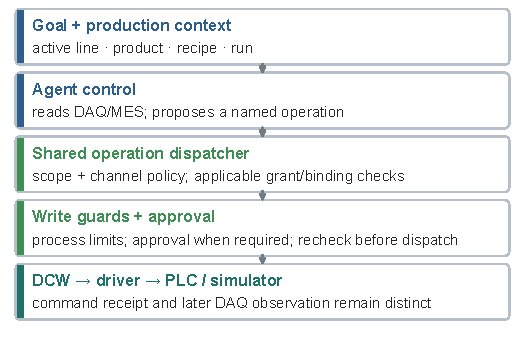
\includegraphics[width=\columnwidth]{resources/fig-agent-control.pdf}
\caption{Agent-control path for a configured industrial task. The agent uses
DAQ/MES context, passes shared operation checks, and routes writes through
process guards, conditional approval, and a pre-dispatch context recheck. DCW
and configured drivers provide device access; command receipts and later
process observations remain separate. The framework does not prescribe an
optimization policy.}
\label{fig:control-path}
\end{figure}

AgentWorkShop implements this path as a modular task-to-device framework.
Registered harnesses connect collaborative tasks to production context, MES
data, analysis and modeling services, DAQ/DCW nodes, and protocol-specific
drivers. Command-line, web, software development kit (SDK), Representational
State Transfer (REST), Model Context Protocol (MCP), and Agent-to-Agent (A2A)
interfaces serve different callers. Task and chat requests enter the
collaboration runtime; direct REST calls reach the shared dispatcher without
creating a task. Scene blueprints define signal maps, objectives, and guards,
while channel profiles, tool policies, and agent bindings scope operations.
The framework supplies this execution path without selecting routes
autonomously or prescribing an optimization strategy. Fig.~\ref{fig:arch}
shows the architecture, and Fig.~\ref{fig:runtime} traces a task through it.

The route study covers three caller routes---registered harness,
fixture-backed command-line task, and direct REST---across the two simulator
mappings. Within the registered-harness route, a fixed-request replay
separates route execution from model selection. A mock-state experiment tests
the approval-bound context check before software dispatch. A separate replay
onboards one documented coating-line blueprint with Modbus TCP and MES REST
interfaces. Four additional simulator scenarios record deterministic
operation calls and process responses for injection molding, wastewater
treatment, annealing, and biaxially oriented polyethylene terephthalate
(BOPET) film. The evidence is limited to these selected paths, one onboarding
configuration, and four scenario-specific control sequences.

This paper makes two contributions. First, it implements a modular execution
path that combines scene configuration, harness adapters, named operations,
shared checks, configured drivers, and service-owned records. For approved
recipe actions, approval is bound to the active line--product--recipe--run
tuple and rechecked just before software dispatch; this check is not an atomic
lock across device I/O. Second, it evaluates route-specific record continuity
for registered-harness tasks under model-mediated and fixed-request
conditions, fixture-backed command-line tasks, and direct REST calls across
two simulator mappings. It also reports four scenario-specific missions, one
coating-line onboarding replay, and a mock-state guard and ablation. Process
readings are reported separately from route-integration outcomes.

Section~II reviews related work. Section~III presents the design rationale,
architecture, and execution flow; Section~IV describes module functions and
integration. Section~V reports the experimental protocol and results,
Section~VI discusses evidence limits, and Section~VII concludes the paper.
